 \section{\label{sec:preliminaries}Theoretical preliminaries}

\subsection{Portfolio optimization problem}

Portfolio optimization is the problem of selecting a set of assets that provides a favorable trade-off between expected return and risk. In the classical mean--variance framework introduced by Markowitz, the return of a portfolio is quantified by the expected return of the selected assets, while the risk is quantified by the variance of the portfolio return~\cite{Markowitz1952,Markowitz1959}. Let $n$ denote the number of available assets, let $\mu_i$ be the expected return of asset $i$, and let $\Sigma_{ij}$ be the covariance matrix of asset returns. In the binary formulation considered here each asset is represented by a variable $x_i\in\{0,1\}$, where $x_i=1$ means that asset $i$ is included in the portfolio. We consider a fixed-cardinality problem, where the number of selected assets is fixed as
\begin{equation}
\sum_{i=1}^{n} x_i = k ,
    \label{eq:cardinality}
\end{equation}
so that the feasible configurations are bit strings of Hamming weight $k$.

The Markowitz objective combines a risk term and a return term. For a binary portfolio $x=(x_1,\ldots,x_n)$ we write the cost function as
\begin{equation}
C(x) = q \sum_{i,j=1}^{n} \Sigma_{ij} x_i x_j - (1-q)\sum_{i=1}^{n} \mu_i x_i ,
    \label{eq:portfolio-cost}
\end{equation}
where $q\in[0,1]$ is the risk-aversion parameter. The first term penalizes portfolios with large return variance, including correlations between assets, while the second favors assets with larger expected return. Minimizing Eq.~\eqref{eq:portfolio-cost} therefore selects portfolios that balance risk against return. With equal weights $1/k$ on the selected assets the two terms carry prefactors $1/k^{2}$ and $1/k$, and it is that normalisation,
% CONFIRMAR contra o codigo
\begin{equation}
C(x) = \frac{q}{k^{2}}\sum_{i,j=1}^{n}\Sigma_{ij}x_ix_j -\frac{1-q}{k}\sum_{i=1}^{n}\mu_ix_i ,
    \label{eq:portfolio-cost-normalised}
\end{equation}
that is used throughout Sec.~\ref{sec:results}. The model defines a quadratic unconstrained binary optimization problem once the cardinality constraint is either enforced by a penalty term or incorporated directly into the feasible subspace~\cite{Lucas2014,Venturelli2019}. This is an equal-weight binary selection version of the Markowitz problem, and should be distinguished from the continuous-weight formulation in which the portfolio weights themselves are optimized.

\subsection{QAOA algorithm}

Let $x\in\{0,1\}^n$ be a binary configuration. A diagonal cost Hamiltonian is defined by
\begin{equation}
H_C = \sum_{x\in\{0,1\}^n} C(x)\ket{x}\bra{x},
    \label{eq:cost-hamiltonian}
\end{equation}
and a QAOA-type variational state of depth $p$ is
\begin{equation}
\ket{\psi_p(\boldsymbol{\gamma},\boldsymbol{\beta})} = \prod_{\ell=1}^{p} e^{-i\beta_\ell H_M} e^{-i\gamma_\ell H_C} \ket{\psi_0},
    \label{eq:qaoa-type-state}
\end{equation}
where $H_M$ is a mixer Hamiltonian and $(\boldsymbol{\gamma},\boldsymbol{\beta})$ are optimized classically~\cite{Farhi2014,Cerezo2021,Blekos2024}.

For a fixed-cardinality portfolio problem the feasible set is
\begin{equation}
\F_{n,k} = \Bigl\{ x\in\{0,1\}^{n}: \textstyle\sum_{j}x_j=k \Bigr\},
    \label{eq:feasible-set}
\end{equation}
and the feasible subspace is $\mathcal{H}_{\F}=\operatorname{span}\{\ket{x}:x\in\F_{n,k}\}$. We write $\F\equiv\F_{n,k}$ when $n$ and $k$ are clear from context. A feasible ansatz satisfies
\begin{equation}
\ket{\psi_0}\in\mathcal{H}_{\F}, \qquad e^{-i\beta H_M}\mathcal{H}_{\F} \subseteq \mathcal{H}_{\F} .
    \label{eq:feasible-condition}
\end{equation} \gabriel{Interestingly, we're not working under the usual adiabatic theorem assumptions that the initial state is the ground state for the mixer. Maybe it's worth mentioning this.}
This is the constraint-preserving strategy of the quantum alternating operator ansatz~\cite{Hadfield2019}, which avoids imposing the hard constraint through energy penalties. For $x = (x_1,\dots,x_n) \in \{0,1\}^n$, we define its support as $\operatorname{supp}(x) = \{i \mid x_i = 1\}$. Recalling the symmetric difference of sets $A \Delta B = (A \setminus B) \cup (B \setminus A) = (A \cup B) \setminus (A \cap B)$, we have $\operatorname{supp}(x) \Delta \operatorname{supp}(y) = \{i \mid x_i \neq y_i\}$; that is, the set of indices where $x$ and $y$ differ.


\subsection{\label{subsec:qwoa-general}Quantum walk optimization ansatz}

A feasible ansatz of the form \eqref{eq:feasible-condition} is completely specified by the pair $(\ket{\psi_0},H_M)$ restricted to $\mathcal{H}_{\F}$. The quantum walk optimization ansatz (QWOA)~\cite{Marsh2019,Marsh2020} makes this restriction explicit by generating the mixer from a continuous-time quantum walk on a graph whose vertices are the feasible solutions themselves.

Let $G_{\F}=(\F,E_{\F})$ be an undirected graph whose vertex set is $\F$ and whose edges are unordered pairs of feasible configurations. Assigning a positive hopping amplitude $w_{xy}=w_{yx}>0$ to each edge, the weighted adjacency operator is
\begin{equation}
\mathcal{A}_{\F} = \sum_{\{x,y\}\in E_{\F}} w_{xy}\bigl(\ket{x}\bra{y}+\ket{y}\bra{x}\bigr),
    \label{eq:feasible-adjacency}
\end{equation}
which reduces to the ordinary adjacency matrix for $w_{xy}\equiv1$. By construction $\mathcal{A}_{\F}$ is Hermitian and supported on $\mathcal{H}_{\F}$, so it satisfies Eq.~\eqref{eq:feasible-condition} for every $\beta\in\mathbb{R}$. The QWOA state of depth $p$ is
\begin{equation}
\bigl|\psi_p^{\mathrm{QWOA}}\bigr\rangle = \prod_{\ell=1}^{p} e^{-i\beta_\ell \mathcal{A}_{\F}} e^{-i\gamma_\ell H_C} \ket{s_{\F}},
    \label{eq:qwoa-state}
\end{equation}
with the uniform feasible superposition
\begin{equation}
\ket{s_{\F}} = |\F|^{-1/2} \sum_{x\in\F}\ket{x}
    \label{eq:uniform-feasible-state}
\end{equation}
as initial state. For $\F_{n,k}$ this is the Dicke state
\begin{equation}
\ket{D^{n}_{k}} = \binom{n}{k}^{-1/2} \sum_{x\in\F_{n,k}}\ket{x} = \ket{s_{\F_{n,k}}} ,
    \label{eq:dicke-state}
\end{equation}
which is efficiently preparable~\cite{Bartschi2019}. The unitary $e^{-i\gamma H_C}$ is diagonal and acts on $\mathcal{H}_{\F}$ only through the values $C(x)$, so all the freedom in the ansatz resides in the graph $G_{\F}$ and the weights $w_{xy}$.

Two structural remarks are useful. First, $G_{\F}$ must be connected, or the reachable set is confined to the connected component containing the support of $\ket{s_\F}$. Second, candidate graphs are usually taken to be regular, because $\ket{s_\F}$ is an eigenvector of $\mathcal{A}_{\F}$ if and only if $G_\F$ is of constant weighted degree. For a non-regular graph the mixer displaces amplitude towards high-degree vertices even in the absence of a cost term, biasing the search by a property of the graph rather than of the objective function.

\subsection{\label{subsec:graph-zoo}Graph families}

The mixers compared in this work differ only in the feasible graph $G_{\F}$ entering Eq.~\eqref{eq:feasible-adjacency}. We collect here the families that appear. Throughout, $d_H(x,y)$ is the Hamming distance between bit strings and $\operatorname{supp}(x)=\{i:x_i=1\}$ \gabriel{repeated definition, already in II.B}.

\paragraph*{Hypercube.} The $n$-dimensional hypercube $Q_n$ has vertex set
$\{0,1\}^{n}$, with $x\sim y$ when $d_H(x,y)=1$. It is $n$-regular, bipartite, of diameter $n$, and distance-transitive. Its vertex set is the whole configuration space, so a walk on $Q_n$ does not respect the cardinality constraint. Figure~\ref{fig:graphs}(a) shows $Q_4$.

\paragraph*{Johnson graph.} For $1\le k\le n-1$, the Johnson graph $J(n,k)$
has vertex set $\F_{n,k}$, with $x\sim y$ when the corresponding $k$-subsets differ in exactly one element, equivalently when $d_H(x,y)=2$. It is $k(n-k)$-regular of diameter $\min(k,n-k)$, and is distance-transitive. Figure~\ref{fig:graphs}(b) shows $J(4,2)$, the octahedron.

\paragraph*{Complete feasible graph.} The complete graph $K_{\F}$ joins every
pair of distinct feasible configurations. It is $(|\F|-1)$-regular with diameter one, and retains no information about which configurations are close in Hamming distance; Fig.~\ref{fig:graphs}(d) shows $K_{\F}$ for $n = 4, \; k = 2$.

\paragraph*{Cyclic graph.} The cycle $C_n$ has vertex set $ [n] = \{0,1,\dots,n-1\}$, with
$i\sim j$ when $j\equiv i\pm1\pmod n$. It is $2$-regular, vertex-transitive, of diameter $\lfloor n/2\rfloor$.

\paragraph*{Johnson-scheme graphs.} The Johnson scheme on $\F_{n,k}$
partitions pairs of vertices by the subset distance
\begin{equation}
d_J(x,y)=k-|\operatorname{supp}(x)\cap\operatorname{supp}(y)| ,
    \label{eq:johnson-distance}
\end{equation}
giving classes $A_1,\dots,A_{r_{\max}}$ with $r_{\max}=\min(k,n-k)$, where $A_r$ is regular of degree $\binom{k}{r}\binom{n-k}{r}$ with edges defined by the relation
\begin{equation}
x \sim y \iff d_J(x,y) = r.
\end{equation} \gabriel{I think there's a lot of abuse of notation making things confusing here. Essentially, we look at the classes as graphs, all on the same vertex set, with different edge sets. It's important for the reader to see they're defined over the same vertex set to understand the definition of $A_T$ below. Ultimately the important point is that $A_r$ = graph of feasible solutions with edges between solutions that differ by exactly $r$ in subset distance and this isn't that clear from the way it's written.}
Consequently, $A_1=J(n,k)$. For non-empty $T\subseteq\{1,\dots,r_{\max}\}$ let $A_T=\bigcup_{r\in T}A_r$. Each $A_T$ is regular of degree $\sum_{r\in T}\binom{k}{r}\binom{n-k}{r}$ and vertex-transitive, with $A_{\{1\}}=J(n,k)$ and $A_{\{1,\dots,r_{\max}\}}=K_{\F}$. The $2^{r_{\max}}-1$ graphs $A_T$ are the family swept in Sec.~\ref{sec:results} \gabriel{Do we know whether this graph family is already known in the graph theory literature?}.

For brevity we write $R_{j_1\cdots j_m}$ for $A_T$ with $T=\{j_1,\dots,j_m\}$, so that $R_1=A_{\{1\}}=J(n,k)$ and $R_{1\cdots r_{\max}}=A_{\{1,\dots,r_{\max}\}}=K_{\F}$; the single class $R_{r_{\max}}$ is \gabriel{known as (otherwise it feels very weird to define hypercubes and cyclic graphs but to give no definition for this way less known family)} the Kneser graph, which for $2k\le n$ joins disjoint $k$-subsets and has degree $\binom{n-k}{k}$. This is the notation used in the axis labels of Figs.~\ref{fig:grid12}--\ref{fig:depth20}.

Table~\ref{tab:graph-zoo} summarizes the parameters. \gabriel{This sentence feels disjointed from everything else around it. And which parameters?}

\begin{table}[b]
\caption{\label{tab:graph-zoo}Feasible graphs used in this work, with
$M=\binom{n}{k}$. The graph $G_{\F}[C_n]$ of the ring $XY$ mixer is not regular; $b(x)$ is the number of maximal cyclic blocks of ones in $x$. \gabriel{Changing the table to the top [t] might make this less cramped with the proof text.}}
\begin{ruledtabular}
\begin{tabular}{lccc}
Graph & Vertices & Degree & Diameter \\
\colrule
$Q_n$ & $2^n$ & $n$ & $n$ \\
$J(n,k)$ & $M$ & $k(n-k)$ & $\min(k,n-k)$ \\
$G_{\F}[C_n]$ & $M$ & $2b(x)$ & -- \\ % CONFIRMAR: preencher o diametro
$K_{\F}$ & $M$ & $M-1$ & $1$ \\
\end{tabular}
\end{ruledtabular}
\end{table}

We do not consider graphs sparser than $J(n,k)$ for the simulations performed in Sec.~\ref{sec:results} because there are none available \gabriel{as we will show below in Proposition 1}: every graph on $\F_{n,k}$ invariant under permutations of the assets is one of the $A_T$, and none of them has smaller degree at the sizes considered here. We only consider permutation-invariant graphs because we are not choosing any particular set of distinguished vertices.

\begin{proposition}
\label{prop:min-degree}
Let $1\le k\le n-1$ and let $S_n$ act on $\F_{n,k}$ by permuting the $n$ assets. Write $r_{\max}=\min(k,n-k)$ and
\begin{equation}
v_j=\binom{k}{j}\binom{n-k}{j},\qquad 1\le j\le r_{\max}.
    \label{eq:valency}
\end{equation}
Let $\Gamma$ be a graph on $\F_{n,k}$, with at least one edge, invariant under this action. Then:
\begin{enumerate}
\item[(i)] $\Gamma=A_T$ for a unique non-empty
$T\subseteq\{1,\dots,r_{\max}\}$;
\item[(ii)] $\Gamma$ is vertex-transitive, hence regular, of degree
$\sum_{j\in T}v_j$;
\item[(iii)] $\deg\Gamma\ \ge\ d_{\min}(n,k):=\min\bigl\{\,k(n-k),\
v_{r_{\max}}\,\bigr\}$, with equality if and only if $T=\{1\}$ or $T=\{r_{\max}\}$, whichever attains the minimum, or either when the two coincide.
\end{enumerate}
In particular $d_{\min}(n,k)=k(n-k)=\Theta(n)$ for fixed $k\ge3$ and $n\ge k^{2}$, and for $k=2$ and $n\ge7$, so no family of $S_n$-invariant graphs on $\F_{n,k}$ has bounded degree as $n$ grows.
\end{proposition}

\begin{proof}

\emph{(i)} Fix a pair $(x,y)$ in $\F_{n,k}$ and set $j=d_J(x,y)=k-|x\cap y|$ \gabriel{to be pedantic, you're missing supps here}. Sorting the indices of $[n]$ according to whether they lie in $x$, in $y$, in both, or in neither splits $[n] = \{0,1,\dots n-1\}$ into four blocks,
\begin{equation*}
\underbrace{\operatorname{supp}(x)\cap \operatorname{supp}(y)}_{k-j},\qquad \underbrace{\operatorname{supp}(x) \setminus \operatorname{supp}(y)}_{j},\qquad
\end{equation*}
\begin{equation*}
\underbrace{\operatorname{supp}(y) \setminus \operatorname{supp}(x)}_{j},\qquad \underbrace{[n]\setminus(\operatorname{supp}(x) \cup \operatorname{supp}(y))}_{n-k-j},
\end{equation*}
where the sizes follow from $|\operatorname{supp}(x)|=|\operatorname{supp}(y)|=k$ and are written beneath each block. Note that all four are determined by $j$ alone.

Now take a second pair $(x',y')$ with the same value of $j$. Its four blocks have the same four sizes, so we may choose a bijection of $[n]$ sending each block of the first pair onto the corresponding block of the second; any such bijection is a permutation $\sigma\in S_n$ \gabriel{While I'm pretty convinced this is true I'm not certain it's that trivial. It definitely doesn't follow from the block cardinalities being equal, because the bijections could not all be "compatible" in the sense that they glue together to form a permutation}with $\sigma(\operatorname{supp}(x))=\operatorname{supp}(x')$ and $\sigma(\operatorname{supp}(y))=\operatorname{supp}(y')$. Conversely, a permutation cannot change $|\operatorname{supp}(x) \cap \operatorname{supp}(y)|$, hence cannot change $j$. The two pairs therefore lie in the same $S_n$-orbit if and only if they share the same $j$, so the orbits of $S_n$ on $\F_{n,k}\times\F_{n,k}$ are indexed precisely by $j$. The range of $j$ is $\{0,\dots,r_{\max}\}$: the fourth block has non-negative size, which forces $j\le n-k$, and $j\le k$ by definition.

A graph invariant under $S_n$ has an edge set closed under the action, so it is a union of each of these orbits \gabriel{It might make the argument a little clearer to explicitly point out that the orbits are essentially the graphs $A_j$ at some point}. It follows now by definition that any graph invariant under $S_n$ must be some $A_T$ with $\emptyset\neq T\subseteq\{1,\dots,r_{\max}\}$.

\medskip \emph{(ii)} $S_n$ acts transitively on $\F_{n,k}$, since any $k$-subset can be mapped to any other, so the graph is vertex-transitive, proving its regularity. To count the neighbours of a fixed $x$ in $A_j$, observe that a vertex $y$ at distance $j$ is obtained by removing $j$ of the $k$ elements of $x$ and inserting $j$ of the $n-k$ elements outside it, these two choices being independent. This gives $v_j=\binom{k}{j}\binom{n-k}{j}$ as in~\eqref{eq:valency}. Distinct $j$ give disjoint neighbourhoods, so the degree of $A_T$ is $\sum_{j\in T}v_j$.

\medskip \emph{(iii)} These degrees $v_j$ satisfy
\begin{equation}
\frac{v_{j+1}}{v_j}=\frac{(k-j)(n-k-j)}{(j+1)^{2}}, \qquad 0\le j<r_{\max}.
    \label{eq:ratio}
\end{equation}
As $j$ increases these ratios strictly decrease. Consequently, over the range $1\le j\le r_{\max}$ the minimum of $v_j$ is attained at one of the two ends:
\begin{equation*}
\min_{1\le j\le r_{\max}} v_j =\min\bigl\{v_1,\;v_{r_{\max}}\bigr\}, \qquad v_1=k(n-k).
\end{equation*}
Since every $v_j$ is positive, any union satisfies $\sum_{j\in T}v_j\ge\min_j v_j$, with equality precisely when $T$ is the singleton achieving that minimum. This is $d_{\min}(n,k)$.

\medskip For $k\le n-k$ we have $v_{r_{\max}}=\binom{n-k}{k}$, and the standard bound $\binom{m}{k}\ge(m/k)^{k}$ shows this grows like a $k$-th power of $n-k$, whereas $v_1=k(n-k)$ grows linearly. The Kneser end is therefore the smaller one only for $n$ close to $2k$; explicitly, $v_{r_{\max}}\ge v_1$ holds for all $n\ge k^{2}$ when $k\ge3$, and for all $n\ge7$ when $k=2$. For the sizes used in this work, $(n,k)=(12,3)$, $(16,4)$ and $(20,5)$, the minimum is $v_1=k(n-k)$, attained by $J(n,k)$. \gabriel{This last sentence doesn't feel like it should be inside the proof. Maybe move it outside along with a short explanation on why the $d_{min}$ estimates and degree bound are useful to us?}
\end{proof}

% =====================================================================
%  FIGURE 1 -- feasible graphs, 2x2 grid, full width
%
%  Panels (b) to (d) share one vertex layout: the six weight-two strings
%  sit on a circle, ordered so that complementary pairs are antipodal.
%  J(4,2) is then the hexagon perimeter plus the two inscribed triangles,
%  and the three absent edges are exactly the long diagonals.
% =====================================================================

% shared vertex positions for panels (b)-(d)
\newcommand{\FeasibleCoords}{%
\coordinate (va) at (90:1.55); % 1100 \coordinate (vb) at (30:1.55); % 0101 \coordinate (vc) at (-30:1.55); % 1001 \coordinate (vd) at (-90:1.55); % 0011 \coordinate (ve) at (-150:1.55); % 1010 \coordinate (vf) at (150:1.55); % 0110 }
\newcommand{\FeasibleLabels}{%
\node[glab] at (90:2.02) {1100}; \node[glab] at (30:2.02) {0101}; \node[glab] at (-30:2.02) {1001}; \node[glab] at (-90:2.02) {0011}; \node[glab] at (-150:2.02) {1010}; \node[glab] at (150:2.02) {0110}; }
\newcommand{\FeasibleDots}{%
\foreach \v in {va,vb,vc,vd,ve,vf} \node[gvert] at (\v) {}; }

\begin{figure*}[t]
\centering
\tikzset{ gvert/.style={circle, draw=black, fill=white, line width=0.5pt, inner sep=0pt, minimum size=4.4pt}, ghub/.style ={circle, draw=black, fill=black!25, line width=0.5pt, inner sep=0pt, minimum size=5.6pt}, qvert/.style={circle, draw=black, fill=white, line width=0.4pt, inner sep=0pt, minimum size=3.4pt}, qfeas/.style={circle, draw=black, fill=black!30, line width=0.4pt, inner sep=0pt, minimum size=4.2pt}, gedge/.style={line width=0.65pt, black!80}, gcut/.style ={line width=0.55pt, black!35, densely dashed}, qedge/.style={line width=0.35pt, black!45}, glab/.style ={font=\scriptsize\ttfamily, inner sep=0.5pt}, wlab/.style ={font=\scriptsize, inner sep=1pt}, panlab/.style={font=\small} }

% ================= (a)  Q_4 graded by Hamming weight =================
\begin{minipage}[t]{0.48\textwidth}
\centering
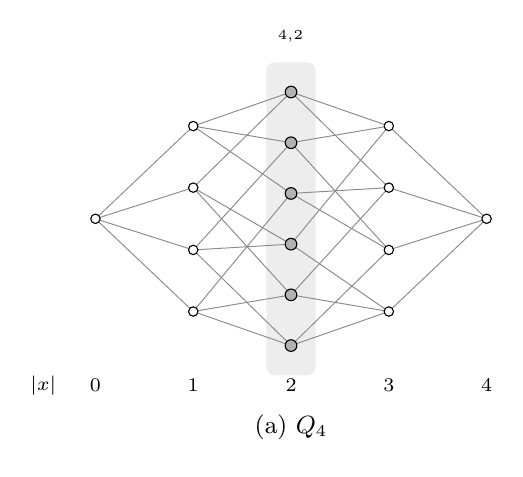
\begin{tikzpicture}[scale=0.92]
  % layer x positions and vertex y positions
\coordinate (w0) at (0,0); \foreach \y/\n in {1.28/1000, 0.43/0100, -0.43/0010, -1.28/0001} \coordinate (\n) at (1.35,\y); \foreach \y/\n in {1.75/1100, 1.05/1010, 0.35/1001, -0.35/0110, -1.05/0101, -1.75/0011} \coordinate (\n) at (2.70,\y); \foreach \y/\n in {1.28/1110, 0.43/1101, -0.43/1011, -1.28/0111} \coordinate (\n) at (4.05,\y); \coordinate (w4) at (5.40,0);

  % shaded band behind the feasible layer
\fill[black!7, rounded corners=3pt] (2.70-0.34,-2.16) rectangle (2.70+0.34,2.16);

  % edges, weight 0 -> 1
\foreach \n in {1000,0100,0010,0001} \draw[qedge] (w0) -- (\n);
  % weight 1 -> 2
\foreach \a/\b in {1000/1100, 1000/1010, 1000/1001, 0100/1100, 0100/0110, 0100/0101, 0010/1010, 0010/0110, 0010/0011, 0001/1001, 0001/0101, 0001/0011} \draw[qedge] (\a) -- (\b);
  % weight 2 -> 3
\foreach \a/\b in {1100/1110, 1100/1101, 1010/1110, 1010/1011, 1001/1101, 1001/1011, 0110/1110, 0110/0111, 0101/1101, 0101/0111, 0011/1011, 0011/0111} \draw[qedge] (\a) -- (\b);
  % weight 3 -> 4
\foreach \n in {1110,1101,1011,0111} \draw[qedge] (\n) -- (w4);

  % vertices
\node[qvert] at (w0) {}; \foreach \n in {1000,0100,0010,0001} \node[qvert] at (\n) {}; \foreach \n in {1100,1010,1001,0110,0101,0011} \node[qfeas] at (\n) {}; \foreach \n in {1110,1101,1011,0111} \node[qvert] at (\n) {}; \node[qvert] at (w4) {};

  % weight axis
\foreach \x/\t in {0/0, 1.35/1, 2.70/2, 4.05/3, 5.40/4} \node[wlab] at (\x,-2.30) {$\t$}; \node[wlab] at (-0.72,-2.30) {$|x|$}; \node[wlab] at (2.70,2.52) {$\F_{4,2}$}; \node[panlab] at (2.70,-2.88) {(a) $Q_4$};
\end{tikzpicture}
\end{minipage}
\hfill
% ================= (b)  Johnson graph J(4,2) =========================
\begin{minipage}[t]{0.48\textwidth}
\centering
\begin{tikzpicture}[scale=0.92]
\FeasibleCoords
  % hexagon perimeter
\foreach \a/\b in {va/vb, vb/vc, vc/vd, vd/ve, ve/vf, vf/va} \draw[gedge] (\a) -- (\b);
  % the two inscribed triangles
\draw[gedge] (va) -- (vc) -- (ve) -- cycle; \draw[gedge] (vb) -- (vd) -- (vf) -- cycle; \FeasibleDots \FeasibleLabels
  % inset: connectivity graph K_4 on the four qubits
  \begin{scope}[shift={(2.62,1.86)}, scale=0.30]
\coordinate (q1) at (0,0); \coordinate (q2) at (1,0); \coordinate (q3) at (1,1); \coordinate (q4) at (0,1); \foreach \a/\b in {q1/q2,q2/q3,q3/q4,q4/q1,q1/q3,q2/q4} \draw[qedge] (\a) -- (\b); \foreach \v in {q1,q2,q3,q4} \node[qvert] at (\v) {};
  \end{scope}
\node[font=\scriptsize] at (2.77,1.50) {$K_4$}; \node[panlab] at (0,-2.88) {(b) $J(4,2)$};
\end{tikzpicture}
\end{minipage}

\vspace{0.9em}

% ================= (c)  ring XY graph  ===============================
\begin{minipage}[t]{0.48\textwidth}
\centering
\begin{tikzpicture}[scale=0.92]
\FeasibleCoords
  % edges of J(4,2) that the cycle does not induce
\foreach \a/\b in {va/vc, vd/vf, va/vf, vc/vd} \draw[gcut] (\a) -- (\b);
  % edges of G_F[C_4]
\foreach \a/\b in {va/vb, vb/vc, vd/ve, ve/vf, va/ve, vc/ve, vb/vd, vb/vf} \draw[gedge] (\a) -- (\b); \foreach \v in {va,vc,vd,vf} \node[gvert] at (\v) {}; \foreach \v in {vb,ve} \node[ghub] at (\v) {}; \FeasibleLabels
  % inset: connectivity graph C_4
  \begin{scope}[shift={(2.62,1.86)}, scale=0.30]
\coordinate (q1) at (0,0); \coordinate (q2) at (1,0); \coordinate (q3) at (1,1); \coordinate (q4) at (0,1); \foreach \a/\b in {q1/q2,q2/q3,q3/q4,q4/q1} \draw[qedge] (\a) -- (\b); \foreach \v in {q1,q2,q3,q4} \node[qvert] at (\v) {};
  \end{scope}
\node[font=\scriptsize] at (2.77,1.50) {$C_4$}; \node[panlab] at (0,-2.88) {(c) $G_{\F}[C_4]\cong K_{2,4}$};
\end{tikzpicture}
\end{minipage}
\hfill
% ================= (d)  complete feasible graph ======================
\begin{minipage}[t]{0.48\textwidth}
\centering
\begin{tikzpicture}[scale=0.92]
\FeasibleCoords \foreach \a/\b in {va/vb, vb/vc, vc/vd, vd/ve, ve/vf, vf/va} \draw[gedge] (\a) -- (\b); \draw[gedge] (va) -- (vc) -- (ve) -- cycle; \draw[gedge] (vb) -- (vd) -- (vf) -- cycle;
  % the three complementary pairs, bowed so they do not meet at the centre
\draw[gedge] (va) to[ left=10] (vd); \draw[gedge] (vb) to[ left=10] (ve); \draw[gedge] (vc) to[ left=10] (vf); \FeasibleDots \FeasibleLabels \node[panlab] at (0,-2.88) {(d) $K_{\F}$};
\end{tikzpicture}
\end{minipage}

\caption{\label{fig:graphs}Feasible graphs for $n=4$, $k=2$.
(a)~The hypercube $Q_4$ of the transverse-field mixer, with vertices arranged by Hamming weight and the weight-two layer $\F_{4,2}$ shaded. Every edge joins consecutive layers, so the walk leaves the feasible subspace. Panels (b) to (d) have vertex set $\F_{4,2}$ and share the same vertex positions, chosen so that complementary strings are opposite. (b)~The Johnson graph $J(4,2)$ of the complete $XY$ mixer, which is $4$-regular of diameter two; the three absent edges are the complementary pairs. The inset shows the connectivity graph $K_4$ on the four qubits, a different object from the feasible graph in the main panel. (c)~The graph $G_{\F}[C_4]$ of the ring $XY$ mixer, with the four edges of $J(4,2)$ it omits shown dashed. The shaded vertices have degree four and the rest degree two, so the graph is not regular and $\ket{D^4_2}$ is not an eigenvector of the mixer. (d)~The complete feasible graph $K_{\F}$ of the Grover mixer, which retains no Hamming structure.}
\end{figure*}